% Chapter 19 -- Claim: Optimized Portfolios Beat Naive Ones
% Requires: amsmath, amssymb, booktabs, array, tabularx, graphicx, tcolorbox (breakable, skins), hyperref or url.
% Defines the callout box only if the preamble has not.
\providecolor{fenavy}{HTML}{1B2A6B}
\providecolor{feshade}{HTML}{F3F5FA}
\makeatletter
\@ifundefined{callout}{%
  \newtcolorbox{callout}{breakable, enhanced,
    colback=white, colframe=gray!70, boxrule=0.5pt, arc=1mm,
    borderline west={2.5pt}{0pt}{gray!70},
    left=8pt, right=8pt, top=4pt, bottom=4pt}%
}{}
\makeatother

\chapter{Claim: Optimized Portfolios Beat Naive Ones}
\label{ch:19}

In 1952 Harry Markowitz showed how to choose a portfolio by trading expected return against variance. Given each asset's expected return and the covariances between assets, an optimizer finds the mix with the highest return for any level of risk. The idea won a Nobel Prize, founded modern portfolio theory and sits inside nearly every asset-allocation tool sold today.

The catch is that nobody knows the expected returns or the covariances. They have to be estimated from history, and the optimizer treats those estimates as exact. It puts the most weight on the assets whose returns were overestimated by luck and whose risks were underestimated by luck. In 2009 Victor DeMiguel, Lorenzo Garlappi and Raman Uppal ran fourteen optimized strategies against the simplest rule there is, putting an equal share in every asset. None of the fourteen beat it consistently.

This chapter asks whether the decades of repairs that followed (constraints, shrinkage, risk parity, hierarchical clustering) have changed that answer.

By the end of the chapter you will be able to:

\begin{itemize}
  \item compute a portfolio's expected return and variance, and the tangency and global minimum-variance portfolios;
  \item explain why estimation error in expected returns dominates, and show how the optimizer magnifies it when assets are similar;
  \item describe the repairs: constraints, shrinkage, minimum variance and risk budgeting, including risk contributions and equal risk contribution;
  \item judge allocation rules out of sample with the Sharpe ratio, the certainty equivalent and the Jobson--Korkie--Memmel test;
  \item state the strong and weak forms of the claim that optimized portfolios beat 1/N, and summarize the evidence for each;
  \item judge an optimized allocation by comparing it with equal weighting, out of sample and after costs.
\end{itemize}

\section{Foundations: mean-variance optimization and estimation error}
\label{sec:19-foundations}

A portfolio holds weights $\mathbf{w}$ in $N$ assets, with expected excess returns $\boldsymbol{\mu}$ and covariance matrix $\boldsymbol{\Sigma}$. Its expected excess return is $\mathbf{w}'\boldsymbol{\mu}$ and its variance is $\mathbf{w}'\boldsymbol{\Sigma}\mathbf{w}$. Throughout, returns are measured in excess of the Treasury bill rate.

\textbf{Mean-variance optimization.} An investor with risk aversion $\gamma$ maximizes
\begin{equation}
  \mathbf{w}'\boldsymbol{\mu} - \frac{\gamma}{2}\,\mathbf{w}'\boldsymbol{\Sigma}\mathbf{w}, \qquad \text{which gives} \qquad \mathbf{w}^* = \frac{1}{\gamma}\,\boldsymbol{\Sigma}^{-1}\boldsymbol{\mu}
  \label{eq:19-mv}
\end{equation}
The set of portfolios that minimize variance for each target return is the \textbf{efficient frontier}. Two portfolios on it matter most:

\begin{itemize}
  \item The \textbf{tangency portfolio} has the highest Sharpe ratio, equal to $\sqrt{\boldsymbol{\mu}'\boldsymbol{\Sigma}^{-1}\boldsymbol{\mu}}$. Every mean-variance investor holds it, levered up or down with cash:
  \begin{equation}
    \mathbf{w}_T = \frac{\boldsymbol{\Sigma}^{-1}\boldsymbol{\mu}}{\mathbf{1}'\boldsymbol{\Sigma}^{-1}\boldsymbol{\mu}}
    \label{eq:19-tangency}
  \end{equation}
  \item The \textbf{global minimum-variance portfolio} has the lowest variance of any fully invested portfolio. It needs no expected returns at all:
  \begin{equation}
    \mathbf{w}_{MV} = \frac{\boldsymbol{\Sigma}^{-1}\mathbf{1}}{\mathbf{1}'\boldsymbol{\Sigma}^{-1}\mathbf{1}}
    \label{eq:19-minvar}
  \end{equation}
\end{itemize}

\textbf{Estimation error.} The sample mean of a return with volatility $\sigma$, estimated over $T$ years, has a standard error of $\sigma/\sqrt{T}$ (Section~\ref{sec:03-se}). For an industry portfolio with $\sigma = 20\%$ and ten years of data, that is 6.3\% a year, larger than the equity premium itself (Figure~\ref{fig:19-se}). Covariances are estimated much more precisely, because they depend on squared returns rather than on the slow drift of prices. Chopra and Ziemba (1993) found that errors in means are far more costly to an optimizer than errors in variances, which in turn cost more than errors in covariances.

\begin{figure}[htbp]
\centering
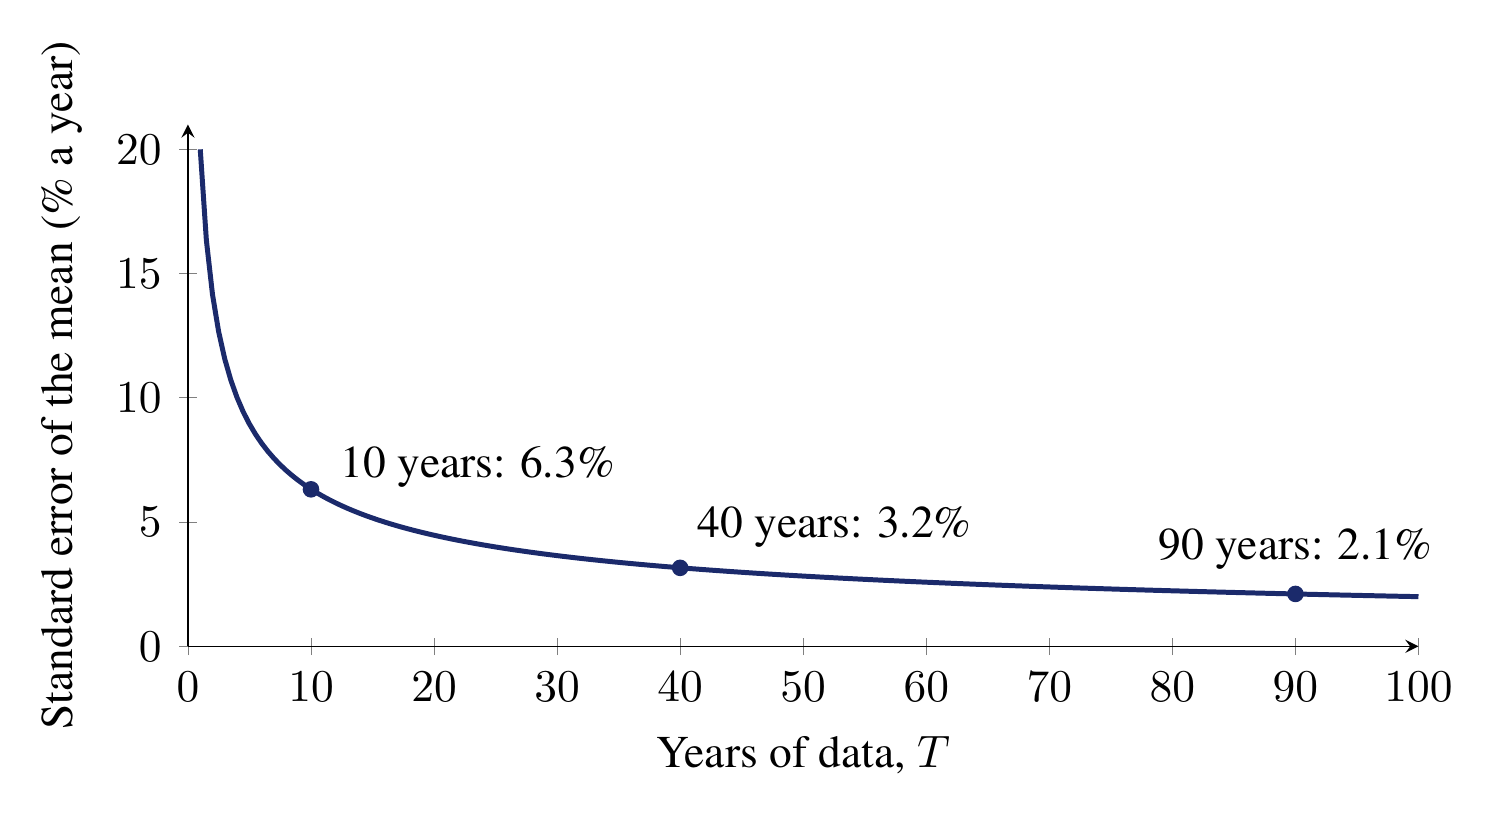
\includegraphics[width=0.85\linewidth]{images/fig19-1-se-years.png}
\caption{The standard error of an average return with 20\% volatility. With ten years of data it is 6.3\% a year; even 90 years leave it at 2.1\%. Differences in expected return between similar assets are far smaller than this, so the optimizer's most important input is mostly noise.}
\label{fig:19-se}
\end{figure}

\textbf{Worked example.} Two assets each have 20\% volatility and correlation 0.5. Asset A is expected to earn 8\% over bills and asset B 6\%. The tangency weights are proportional to $\boldsymbol{\Sigma}^{-1}\boldsymbol{\mu}$, which is proportional to $(0.08 - 0.5 \times 0.06,\; 0.06 - 0.5 \times 0.08) = (0.05,\; 0.02)$. Scaled to sum to 1, that is 71\% in A and 29\% in B.

\begin{itemize}
  \item Suppose the estimates were swapped, A at 6\% and B at 8\%. That is a 2-point error, a third of one standard error. The weights flip to 29\% in A and 71\% in B.
  \item {\sloppy If the correlation is 0.9 instead of 0.5, the original estimates give $(0.08 - 0.054,\; 0.06 - 0.072) = (0.026,\; -0.012)$: \textbf{186\% in A and $-86\%$ in B}.\par}
\end{itemize}

The more alike the assets, the more the optimizer bets on small differences in their estimated returns (Figure~\ref{fig:19-weights}).

\begin{figure}[htbp]
\centering
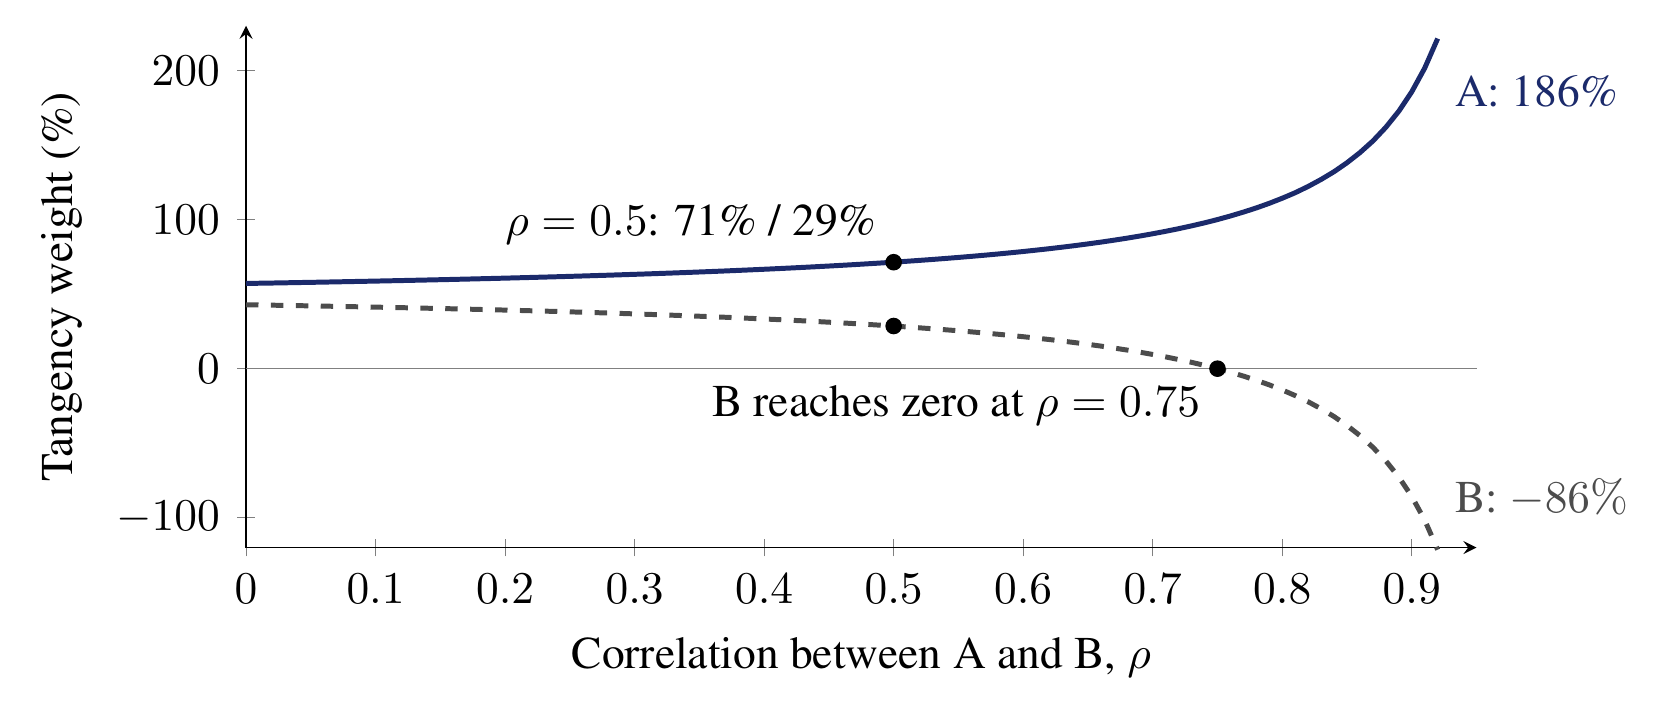
\includegraphics[width=0.85\linewidth]{images/fig19-2-weights-corr.png}
\caption{Tangency weights in the worked example as the correlation between the two assets rises, with expected returns fixed at 8\% and 6\%. At a correlation of 0.5 the split is 71/29; B's weight reaches zero at 0.75; at 0.9 the optimizer holds 186\% in A and shorts 86\% of B.}
\label{fig:19-weights}
\end{figure}

\textbf{Equal weighting (1/N)} puts $1/N$ in each asset. It uses no estimates, so it has no estimation error. It is optimal only if all assets have the same expected return, the same variance and the same pairwise correlations, but it never makes a large mistake.

\textbf{Repairs.} Four families of methods try to keep what optimization gets right while limiting estimation error:

\begin{itemize}
  \item \textbf{Constraints.} Ruling out short sales ($\mathbf{w} \geq 0$) caps the damage a bad estimate can do.
  \item \textbf{Shrinkage.} The Ledoit--Wolf estimator pulls the sample covariance $\mathbf{S}$ toward a simple target $\mathbf{F}$, with the intensity $\delta$ chosen from the data:
  \begin{equation}
    \hat{\boldsymbol{\Sigma}} = \delta\mathbf{F} + (1 - \delta)\mathbf{S}
    \label{eq:19-shrink}
  \end{equation}
  \item \textbf{Ignoring means.} Minimum-variance and risk-based rules drop $\boldsymbol{\mu}$, the noisiest input.
  \item \textbf{Risk budgeting.} Each asset's \textbf{risk contribution} is
  \begin{equation}
    RC_i = \frac{w_i\,(\boldsymbol{\Sigma}\mathbf{w})_i}{\sigma_p}
    \label{eq:19-rc}
  \end{equation}
  and the contributions sum to the portfolio volatility $\sigma_p$. \textbf{Equal risk contribution} sets them equal (Maillard, Roncalli and Teiletche 2010). \textbf{Inverse-volatility weighting} does so exactly when all correlations are equal.
\end{itemize}

\textbf{Judging out of sample.} Portfolios are formed from past data only and judged on the returns that follow. Two measures recur:

\begin{itemize}
  \item the Sharpe ratio;
  \item the \textbf{certainty equivalent}, the risk-free return the investor would accept instead:
  \begin{equation}
    CE = \mu_p - \frac{\gamma}{2}\,\sigma_p^2
    \label{eq:19-ce}
  \end{equation}
\end{itemize}

The \textbf{Jobson--Korkie test} (Jobson and Korkie 1981), with Memmel's (2003) correction, checks whether two Sharpe ratios differ by more than chance.

\textbf{Further reading.} Bodie, Kane and Marcus, \emph{Investments} (optimal risky portfolios and the efficient frontier); Cochrane, \emph{Asset Pricing} (the mean-variance problem in a modern asset-pricing framework); Campbell and Viceira, \emph{Strategic Asset Allocation}, and Meucci, \emph{Risk and Asset Allocation} (estimation error, Bayesian methods and long-horizon allocation); Roncalli, \emph{Introduction to Risk Parity and Budgeting}; Grinold and Kahn, \emph{Active Portfolio Management} (practitioner portfolio construction and transaction costs).

\section{How it works}
\label{sec:19-how}

In theory the mean-variance portfolio is the best one can do: no other mix of the same assets has a higher expected Sharpe ratio. In practice the optimizer is fed estimates, and it cannot tell signal from noise. Richard Michaud (1989) put the problem bluntly. Mean-variance optimization tends to maximize the effects of errors in its inputs, so that unconstrained optimized portfolios can do worse than equal weighting. Fischer Black and Robert Litterman (1992), writing from Goldman Sachs, described quantitative allocation models as difficult to use and prone to producing ``badly behaved'' portfolios.

The mechanism is in the inverse covariance matrix. $\boldsymbol{\Sigma}^{-1}$ magnifies differences between similar assets, as the worked example showed. Ten industry portfolios are all highly correlated with the market, so $\boldsymbol{\Sigma}^{-1}\boldsymbol{\mu}$ is dominated by small, noisy differences in their estimated means. The result is large long and short positions that change sharply from one month to the next. Each change costs money to trade.

The repairs attack different parts of the problem:

\begin{itemize}
  \item \textbf{Drop the means.} Minimum-variance portfolios use only $\boldsymbol{\Sigma}$. They usually lower volatility, but they still invert a noisy matrix and can hold large short positions.
  \item \textbf{Constrain the weights.} Jagannathan and Ma (2003) showed that a no-short-sale constraint is equivalent to shrinking the largest elements of the sample covariance matrix. It helps even when the true optimal portfolio would hold short positions.
  \item \textbf{Shrink the estimates.} Ledoit and Wolf (2004) shrink the sample covariance toward a scaled identity matrix. Black and Litterman (1992) shrink expected returns toward those implied by market equilibrium.
  \item \textbf{Avoid inversion.} Inverse-volatility weighting and equal risk contribution need only volatilities and correlations. \textbf{Hierarchical risk parity} (L\'opez de Prado 2016) clusters assets by correlation and splits capital down the resulting tree, never inverting $\boldsymbol{\Sigma}$.
  \item \textbf{Trade less.} Rebalancing less often, or penalizing turnover, cuts costs at the price of holding stale weights.
\end{itemize}

Each repair moves the portfolio closer to 1/N. That is the central tension of this chapter: the more an optimizer is protected from estimation error, the more it resembles the rule it was meant to beat.

\section{The claim}
\label{sec:19-claim}

\begin{callout}
\textbf{Claim.} Optimized portfolios deliver better out-of-sample risk-adjusted returns than simple rules such as equal weighting.
\end{callout}

The claim comes in two strengths:

\begin{itemize}
  \item \textbf{The strong form} is that classic mean-variance optimization, fed with sample estimates, beats 1/N out of sample.
  \item \textbf{The weak form} is that some disciplined form of optimization beats 1/N reliably, after trading costs. That form might be constrained, shrunk, risk-based or clustered.
\end{itemize}

To count as evidence, a result must:

\begin{itemize}
  \item use only data available at each rebalancing date;
  \item report the Sharpe ratio or certainty equivalent net of realistic costs;
  \item show that the gap over 1/N is larger than chance would produce;
  \item hold across more than one set of assets.
\end{itemize}

\section{The original evidence}
\label{sec:19-evidence}

\textbf{The theory (Markowitz 1952).} Markowitz's paper proves that the mean-variance portfolio is optimal when means and covariances are known. It contains no test, because there is nothing to test in sample. The optimized portfolio always wins on the data used to build it.

\textbf{The warnings (Michaud 1989; Black and Litterman 1992; Chopra and Ziemba 1993).} Practitioners reported early that optimized portfolios were concentrated, unstable and hard to justify to clients. Chopra and Ziemba ranked the damage done by errors in each input and found errors in means to be the most harmful by far. That finding is the reason minimum-variance and risk-based rules exist.

\textbf{The repairs work in their own tests.}

\begin{itemize}
  \item Jagannathan and Ma (2003) found that long-only minimum-variance portfolios built from monthly sample covariances performed about as well as those built from factor models, shrinkage estimators or daily data.
  \item Ledoit and Wolf (2004) derived the optimal shrinkage intensity and showed that the shrunk matrix is well conditioned even when assets outnumber observations.
  \item L\'opez de Prado (2016) reported that hierarchical risk parity delivered lower out-of-sample variance than Markowitz's critical-line algorithm, even though minimum variance is that algorithm's own objective. The evidence in the paper's abstract comes from Monte Carlo experiments, not from market data.
\end{itemize}

\textbf{The challenge (DeMiguel, Garlappi and Uppal 2009).} DeMiguel, Garlappi and Uppal (DGU) evaluated fourteen models across seven empirical datasets, on Sharpe ratio, certainty equivalent and turnover. None was consistently better than 1/N. Their models included:

\begin{itemize}
  \item sample mean-variance;
  \item Bayesian and Bayes--Stein estimators;
  \item minimum variance;
  \item constrained versions of each;
  \item mixtures of several rules.
\end{itemize}

They then asked how long an estimation window would be needed for sample mean-variance to beat 1/N. Their answer was around 3,000 months for 25 assets and about 6,000 months for 50, compared with roughly 1,100 months of U.S. stock data available today.

\textbf{The response (Kirby and Ostdiek 2012).} Kirby and Ostdiek argued that DGU's design favoured 1/N by focusing on portfolios with high estimation risk and extreme turnover. In their tests, standard mean-variance often beat 1/N before costs, but high turnover eroded the advantage. Two simple strategies, \textbf{volatility timing} and \textbf{reward-to-risk timing}, beat 1/N even with high transaction costs. Volatility timing weights assets by inverse variance; reward-to-risk timing weights by the ratio of mean to variance. Both ignore correlations and trade little.

The literature therefore agrees on the strong form: sample mean-variance loses to 1/N. It disagrees on the weak form, and the disagreement turns on costs, turnover and which assets are used.

\section{Replication lab: nine allocation rules against 1/N}
\label{sec:19-lab}

\begin{callout}
\textbf{Lab 19 at a glance.} \emph{Claim on trial:} optimized portfolios beat equal weighting out of sample. \emph{Data:} 10 and 30 industry portfolios and 25 size/book-to-market portfolios from the Kenneth R. French Data Library, with the risk-free rate; free. \emph{Code:} runs as a script (\texttt{python lab19.py}) or as a notebook (\texttt{lab19\_walkthrough.ipynb}) with a prediction prompt before each step.
\end{callout}

Lab 19 runs nine allocation rules walk-forward (Chapter 5). Each month, every rule is estimated on the previous 120 months of value-weighted excess returns and held for one month. Turnover is measured against the weights after they have drifted with that month's returns.

\begin{center}
\small
\begin{tabularx}{0.9\linewidth}{@{}>{\raggedright\arraybackslash}p{0.38\linewidth}>{\raggedright\arraybackslash}X@{}}
\toprule
Rule & What it estimates \\
\midrule
1/N & Nothing \\
Mean-variance (sample) & Means and covariance; scaled to sum to 1, gross exposure capped at 5 \\
Mean-variance, long-only & Means and covariance; risk aversion 5, weights 0 to 1 \\
Minimum variance (sample) & Covariance \\
Minimum variance, long-only & Covariance \\
Minimum variance, Ledoit--Wolf & Shrunk covariance \\
Risk parity (inverse volatility) & Volatilities \\
Equal risk contribution & Covariance \\
Hierarchical risk parity & Correlation clusters and variances \\
\bottomrule
\end{tabularx}
\end{center}

The lab has four parts:

\begin{itemize}
  \item \textbf{Part A} runs all nine rules on the 10 industry portfolios. It reports the Sharpe ratio, the certainty equivalent with $\gamma = 1$, turnover, extreme weights and maximum drawdown. Each rule is tested against 1/N with the Jobson--Korkie--Memmel test (Figures 19.3 and 19.4).
  \item \textbf{Part B} repeats the comparison on 30 industries and on 25 size/book-to-market portfolios, net of 25 basis points per unit of turnover (Figure 19.5).
  \item \textbf{Part C} varies the estimation window (60, 120, 240 months), costs (0, 25, 50 bp) and rebalancing frequency (1, 3, 12 months), and reports returns in three crises (Figure 19.6).
  \item \textbf{Part D} measures how unstable each rule's weights are: gross exposure, the largest weight, the share of short positions and month-to-month weight changes (Figure 19.7).
\end{itemize}

{\sloppy The option \texttt{-{}-fast} drops the three slower constrained rules, and \texttt{python lab19.py -{}-source sim} tests the code on simulated data.\par}

\textbf{What the simulated run shows.} The lab was run end to end only on simulated data. In the simulation every asset has a similar true Sharpe ratio, so 1/N is close to optimal by construction. The results show that the code behaves as theory predicts, not what real markets do.

\begin{itemize}
  \item On ten simulated assets, 1/N earned a Sharpe ratio of 0.44. Sample mean-variance earned 0.30, with average gross exposure of 4.1 and turnover of 74\% a month.
  \item Inverse volatility, equal risk contribution and hierarchical risk parity all landed between 0.44 and 0.45. None differed from 1/N significantly.
  \item Sample minimum variance cut volatility from 16\% to 12\% but earned a lower Sharpe ratio (0.40). Ledoit--Wolf shrinkage recovered most of the gap (0.43).
  \item With 30 or 25 assets, estimation error grew. After costs, sample mean-variance fell to Sharpe ratios of 0.15 and 0.25, and sample minimum variance fell to 0.07 and 0.10. Both were significantly worse than 1/N.
  \item A 240-month window lifted sample mean-variance to 0.44, close to 1/N, and cut its turnover by a third.
\end{itemize}

Run on real data, the lab will answer the question the simulation cannot: whether real assets differ enough in expected return and risk for optimization to earn back its estimation error.

\section{Stress tests}
\label{sec:19-stress}

\textbf{Estimation window.} DGU's critical window for 25 assets, about 3,000 months, is far longer than any real sample. Longer windows reduce estimation noise but use older data, which may no longer describe today's markets. Part C shows how the ranking changes as the window grows from five to twenty years.

\textbf{Trading costs.} Optimized rules trade far more than 1/N. In the simulated run, sample mean-variance turned over 74\% of the portfolio each month, against 3\% for 1/N. At 25 bp per unit of turnover, that difference alone costs about 2\% a year. Any claimed gain from optimization should be judged net of costs at the scale the investor actually trades (Chapter 6).

\textbf{Rebalancing frequency.} Rebalancing quarterly or annually cuts turnover. The weights are then estimated on older data, so the reduction is not free. Part C reports whether the trade-off helps the optimized rules more than 1/N.

\textbf{Asset set.} Optimization should do best when assets differ most. Industry and size/book-to-market portfolios are already diversified and highly correlated with the market, which makes $\boldsymbol{\Sigma}$ nearly singular. Asset classes with genuinely different risks, such as stocks, bonds and commodities, give optimization more to work with. Individual stocks give it less, because the number of parameters grows with the square of the number of assets.

\textbf{Crises.} Minimum-variance portfolios tend to lose less in sell-offs, because they tilt toward low-volatility assets. Part C reports returns in the 2008 crisis, the 2020 crash and 2022 for each rule. A smaller loss in a crisis is a real benefit to some investors even if the Sharpe ratio over the whole sample is no higher.

\textbf{Statistical power.} Sharpe ratios estimated over 90 years still have standard errors of roughly 0.1. A rule would need a large edge over 1/N for the difference to be detectable. Failing to reject equality is not proof that two rules are equally good.

\section{Verdict}
\label{sec:19-verdict}

\begin{callout}
\textbf{Verdict: fails} (as of October 2026). In its plain form the claim fails. Sample mean-variance optimization, the method the claim is built on, does not beat equal weighting out of sample in the published evidence. DGU's estimate of the data needed for it to win, about 3,000 months for 25 assets, exceeds any real sample by a wide margin.
\end{callout}

The repaired versions do better but do not rescue the claim:

\begin{itemize}
  \item Constrained and shrunk minimum-variance portfolios reliably lower volatility. They do not reliably raise the Sharpe ratio above 1/N.
  \item Risk-based rules (inverse volatility, equal risk contribution, hierarchical risk parity) tend to tie with 1/N, which they closely resemble when assets have similar risks.
  \item Kirby and Ostdiek's timing rules are the strongest case for the weak form. They succeed by ignoring correlations and trading little, which is to say by giving up most of what makes optimization optimization.
\end{itemize}

The verdict would change if the lab, run on real data, showed a disciplined optimizer beating 1/N significantly, net of costs, across all three asset sets.

\section{What investors can use}
\label{sec:19-investors}

\begin{itemize}
  \item \textbf{Treat 1/N as the benchmark.} Any optimized allocation should be compared with equal weighting of the same assets, out of sample and net of costs. A strategy that cannot beat it is adding complexity, not value.
  \item \textbf{Distrust the expected-return inputs most.} If an optimizer's output changes sharply when an expected return moves by a percentage point, the output reflects the input, not the market.
  \item \textbf{Use optimization for risk, not return.} Minimum-variance and risk-budgeting tools do what they promise, lowering volatility or balancing risk, without relying on forecasts of returns.
  \item \textbf{Count the turnover.} A gain of a few tenths of a percent a year disappears quickly at 70\% monthly turnover.
  \item \textbf{Prefer constraints you can explain.} Position limits and no-short rules work partly because they are crude.
\end{itemize}

\textbf{Questions to ask a manager who sells optimized portfolios:}

\begin{itemize}
  \item How does the strategy compare with 1/N on the same assets, out of sample and after costs?
  \item Where do the expected returns come from, and how sensitive are the weights to them?
  \item How many parameters are estimated, and from how many observations?
  \item What is the average monthly turnover, and what cost per trade is assumed?
  \item Which constraints are imposed, and how much of the performance comes from them rather than from the optimizer?
\end{itemize}

\begin{callout}
\textbf{What Failed: the optimizer nobody would use.} In the early 1990s Fischer Black and Robert Litterman, working in Goldman Sachs's fixed-income division, reported that quantitative asset-allocation models had not played the important role in global portfolio management that their logic deserved. Investment professionals found the models difficult to use, and the portfolios they produced were ``badly behaved'': concentrated, extreme and sensitive to small changes in inputs. Black and Litterman's fix was to stop trusting historical means. They started from the expected returns implied by market equilibrium and let managers tilt away only where they had confident views. Michaud reached the same diagnosis from the other side: unconstrained optimization maximizes the effects of errors in its inputs. The lesson has outlived both papers. The optimizer works exactly as designed; the problem is what it is fed.
\end{callout}

\section{Open questions}
\label{sec:19-open}

\begin{itemize}
  \item \textbf{Many assets.} With hundreds of stocks, sample covariance matrices become singular. Do newer nonlinear shrinkage and factor-based estimators make large-scale optimization competitive with 1/N?
  \item \textbf{Machine-learning allocations.} Do methods that learn weights directly from data avoid estimation error, or simply hide it in more parameters? Chapter 21 takes up the general question.
  \item \textbf{Cost-aware optimization.} Optimizing net of trading costs, with turnover penalties, changes both the weights and the comparison. How much of DGU's result survives?
  \item \textbf{Diversification in stress.} Risk-based portfolios depend on correlations staying stable. Chapter 20 asks what happens when they do not.
\end{itemize}

\section*{Exercises}
\addcontentsline{toc}{section}{Exercises}

\subsection*{Conceptual (all readers)}

\begin{enumerate}
  \item Two assets have volatilities of 15\% and 25\% and correlation 0.3. Compute the global minimum-variance weights. Then compute the inverse-volatility weights. Which portfolio has lower variance, and by how much?
  \item Using the worked example in Section~\ref{sec:19-foundations}, find the correlation at which the tangency portfolio first takes a short position in asset B, with expected returns of 8\% and 6\%.
  \item An asset has 18\% volatility. How many years of data are needed for the standard error of its mean return to fall below 1\% a year? What does this imply for estimating the difference in mean returns between two industries?
\end{enumerate}

\subsection*{Lab extensions (technical readers)}

\begin{enumerate}
  \setcounter{enumi}{3}
  \item Part A: run on real data. Which rules beat 1/N on Sharpe ratio, and are any differences significant at the 5\% level?
  \item Re-run with \texttt{-{}-window 240} and \texttt{-{}-window 360}. How quickly does sample mean-variance approach 1/N?
  \item Part B: compare the gap between sample minimum variance and its Ledoit--Wolf version on 10, 30 and 25 assets. Why does shrinkage matter more with more assets?
  \item Add a rule that holds half 1/N and half minimum variance, Ledoit--Wolf. Does the mixture beat both parts?
  \item Kirby and Ostdiek argue that DGU's design favoured 1/N. DGU might reply that real investors face exactly that estimation risk. Who has the better of the argument, and what evidence would settle it?
  \item A pension fund holds stocks, bonds, real estate and commodities. Would you expect optimization to do better relative to 1/N for this fund than for a portfolio of ten U.S. industries? Explain.
\end{enumerate}

\section*{References}
\addcontentsline{toc}{section}{References}

\begin{itemize}
  \item Black, F. and Litterman, R. (1992). Global Portfolio Optimization. \emph{Financial Analysts Journal} 48(5): 28--43.
  \item Chopra, V. K. and Ziemba, W. T. (1993). The Effect of Errors in Means, Variances, and Covariances on Optimal Portfolio Choice. \emph{Journal of Portfolio Management} 19(2): 6--11.
  \item DeMiguel, V., Garlappi, L. and Uppal, R. (2009). Optimal versus Naive Diversification: How Inefficient Is the 1/N Portfolio Strategy? \emph{Review of Financial Studies} 22(5): 1915--1953.
  \item Jagannathan, R. and Ma, T. (2003). Risk Reduction in Large Portfolios: Why Imposing the Wrong Constraints Helps. \emph{Journal of Finance} 58(4): 1651--1684.
  \item Jobson, J. D. and Korkie, B. M. (1981). Performance Hypothesis Testing with the Sharpe and Treynor Measures. \emph{Journal of Finance} 36(4): 889--908.
  \item Kirby, C. and Ostdiek, B. (2012). It's All in the Timing: Simple Active Portfolio Strategies That Outperform Naive Diversification. \emph{Journal of Financial and Quantitative Analysis} 47(2): 437--467.
  \item Ledoit, O. and Wolf, M. (2004). A Well-Conditioned Estimator for Large-Dimensional Covariance Matrices. \emph{Journal of Multivariate Analysis} 88(2): 365--411.
  \item L\'opez de Prado, M. (2016). Building Diversified Portfolios That Outperform Out of Sample. \emph{Journal of Portfolio Management} 42(4): 59--69.
  \item Maillard, S., Roncalli, T. and Teiletche, J. (2010). The Properties of Equally Weighted Risk Contribution Portfolios. \emph{Journal of Portfolio Management} 36(4): 60--70.
  \item Markowitz, H. (1952). Portfolio Selection. \emph{Journal of Finance} 7(1): 77--91.
  \item Memmel, C. (2003). Performance Hypothesis Testing with the Sharpe Ratio. \emph{Finance Letters} 1: 21--23.
  \item Michaud, R. O. (1989). The Markowitz Optimization Enigma: Is ``Optimized'' Optimal? \emph{Financial Analysts Journal} 45(1): 31--42.
\end{itemize}

\textbf{Data:} Kenneth R. French Data Library: 10 and 30 Industry Portfolios; 25 Portfolios Formed on Size and Book-to-Market; Fama/French 3 Factors (risk-free rate).
